\documentclass[12pt, spanish]{article}
\usepackage[spanish]{babel}
\selectlanguage{spanish}
\usepackage[utf8]{inputenc}
\usepackage{amsmath}
\usepackage{newfloat}
%\usepackage{fullpage}
\usepackage[top=0.80in, bottom=0.80in, left=0.85in, right=0.85in]{geometry}
\usepackage{multicol}
\usepackage{wrapfig}
\usepackage{enumerate}
\usepackage{graphicx}
\usepackage{newfloat}
\usepackage{geometry}
\usepackage{array}
\usepackage{hyperref}
\usepackage{multirow}
\usepackage{multicol}
\usepackage{float}
\restylefloat{table}
\renewcommand{\baselinestretch}{1.5}
\begin{document}
\title{Ejercitación QGIS}


\thispagestyle{empty}
\begin{center}

\includegraphics[width=15cm]{Universidad_San_Andres_UdeSA.jpg}
\end{center}

	\begin{center}
	\LARGE
\textbf{HERRAMIENTAS COMPUTACIONALES PARA INVESTIGACIÓN}
	

	\vspace{1.5 cm}
	\LARGE
	\textit{Tarea 3}

	\vspace{1 cm}
	\Large
	Clara Pasman \& Rosario Podestá\
	
	\vspace{1.3cm}
	\Large	
	Profesora: Amelia Gibbons\

	
	\vspace{1 cm}
	\normalsize
	\today
	\end{center}
	
\clearpage

\section{Ejercicio 1}
El siguiente gráfico muestra la relación entre la precipitación y la cantidad de hurtos en cada condado del estado de Maryland. No encontramos una correlación clara entre ambas variables. Las zonas de mayor precipitación pesentan una cantidad de hurtos heterogénea. Esto permite pensar en dos posibles hipótesis. La primera indica que la precipitación no determina este tipo de crímenes, poco respaldado por la literatura del crimen. Por otra parte, se abre una serie de posibilidades para encontrar qué es lo que determina el crimen. 

\begin{figure}[hbtp]
\caption{Hurtos per cápita y precipitación}
\centering
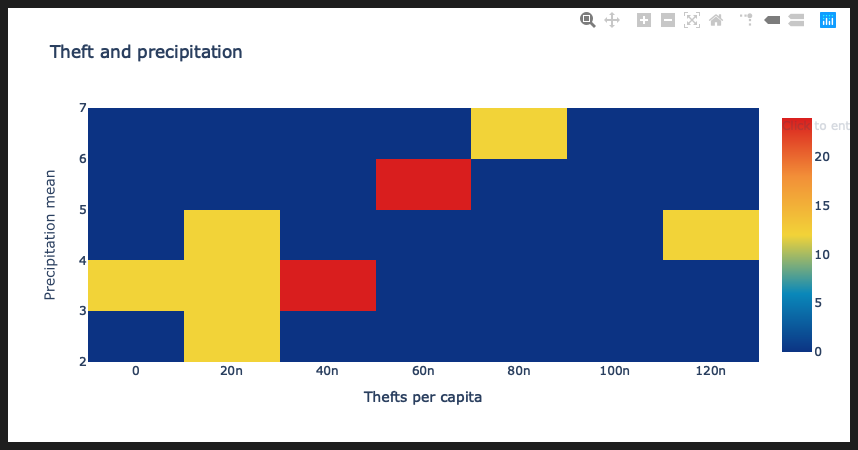
\includegraphics[width=16cm]{grafico 1.png}
\end{figure}
\clearpage

Para observarlo de una manera más dinámica, presentamos el siguiente mapa. La precipitación se observa a través de las tonalidades grises, mientras que los bordes de colores muestran los distintos niveles de hurtos per cápita. La falta de correlación entre dichas variables se observa claramente al presentar distintos niveles de hurto per cápita para disitntos niveles de precipitaciones, especialmente remarcamos la heterogeneidad entre los niveles de hurto n el sudeste del condado, donde los niveles de precipitación son más homogéneos. 

\begin{figure}[hbtp]
\caption{Mapa de Hurtos per cápita y precipitación}
\centering
\includegraphics[width=16cm]{theft y precipitation graph.png}
\end{figure}

\clearpage
\section{Ejercicio 2}

En este caso observamos la correlación entre la cantidad de robos y la proporción de afroamericanos en la población de cada condado. 

\begin{figure}[hbtp]
\caption{Robos per capita y proporción de Afroamericanos}
\centering
\includegraphics[width=16cm]{black y theft.png}
\end{figure}

Observamos que los condados con menor proporción de afroamericanos en su población presentan menores niveles de robos. Esto puede explicarse por menores ingresos que presentan dicho grupo étnico, lo que impulsa la actividad criminal en dichas áreas.


\end{document}
